
\section{Research Process}
Part of any research process is rigorous record keeping to ensure experiments can be independently and reliably reproduced.
While researchers keep meticulous journals, when dealing with software this bookkeeping can be largely automated.


\subsection{Version Control}
Software engineering primarily relies on version control systems, such as GitHub, to keep track of code changes.

....

\subsection{Experiment Tracking}
\begin{figure}[h]
    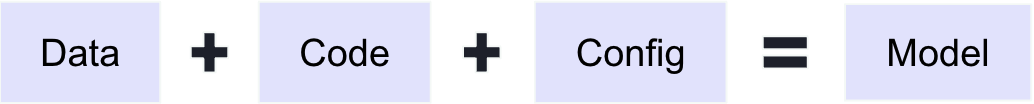
\includegraphics[width=\linewidth]{chapters/NLP/figures/model.png}
    \label{fig:model}
\end{figure}
An experiment is defined by the training code, data, and a configuration file.
When ML and Data Science are involved, the data generating process has to be documented.
In software engineering we say that code doesn't exist until it is "checked into" version control.
Similarly, data doesn't exist until it is stored in the cloud.
In addition to the raw data, we should also store documentation about how it was obtained, by whom, when, and if there have been any additional processing steps.
This should be done in a way that is easy to replicate and understand -- ideally it is documented in code as well.

While version control system are specialized to keep track changes in plain text files, they are not well suited for tracking changes in larger file objects.
To keep track of data (and model) versions the ML community has developed specialized tools\footnote{Weights\&Biases, Neptune}, which we have integrated into Sheepy.
As part of the training run a new experiment is initialized and all hyperparameters are tracked, along with the versions of all dependencies

In addition, these tools allow visualization of metrics, plots, comparison to previous experiments, as well as enables collaboration and sharing of results by directly linking to the tracked experiments.
While being able to repeat previous experiments is important, it is even better if we don't have to -- ML experiments can be expensive.
In addition it is useful to generate formally track \textit{artifacts}, where an artifact refers to a file that is not a code file, but is an important piece of data that is used to generate the results or is the result of an experiment, such as datasets and models.
The file itself is uploaded to a cloud storage service\footnote{Amazon S3, Google Cloud Storage}, and we store a reference to the file as part of the experiment.
Additionally we can store metadata, such as how many samples the data contains, the size and type of fields, when it was created etc..
This facilitates discovery, analysis, iteration, and collaboration.


\subsection{Data Preparation}
One should ensure that all steps necessary to obtain and pre-process the data are documented, ideally in code.
To this end, we provide utilities to handle
\begin{itemize}
    \item Data download
    \item Pre-processing
    \item Splitting into training, validation, and test sets
    \item Feeding data to the model during training
\end{itemize}

We'll go over each of these steps in more detail in the next sections.
The goal is to rerun an experiment from scratch with a single command and we build on top of PyTorch Lightning's DataModule class to handle these steps.
\subsubsection{Data Download}
Downloading the dataset from cloud storage and caching it locally should be part of the training script.

\subsubsection{Data Preprocessing}
In general, pre-processing refers to transformation steps we want to apply to the raw data to make it suitable to input into the model.
In NLP, raw text needs to be translated into arrays of integers that the model can map to embedding vectors (see Section \ref{embeddings}) -- we call this process tokenization (Fig. \ref{fig:tokenization}).
\begin{figure}
    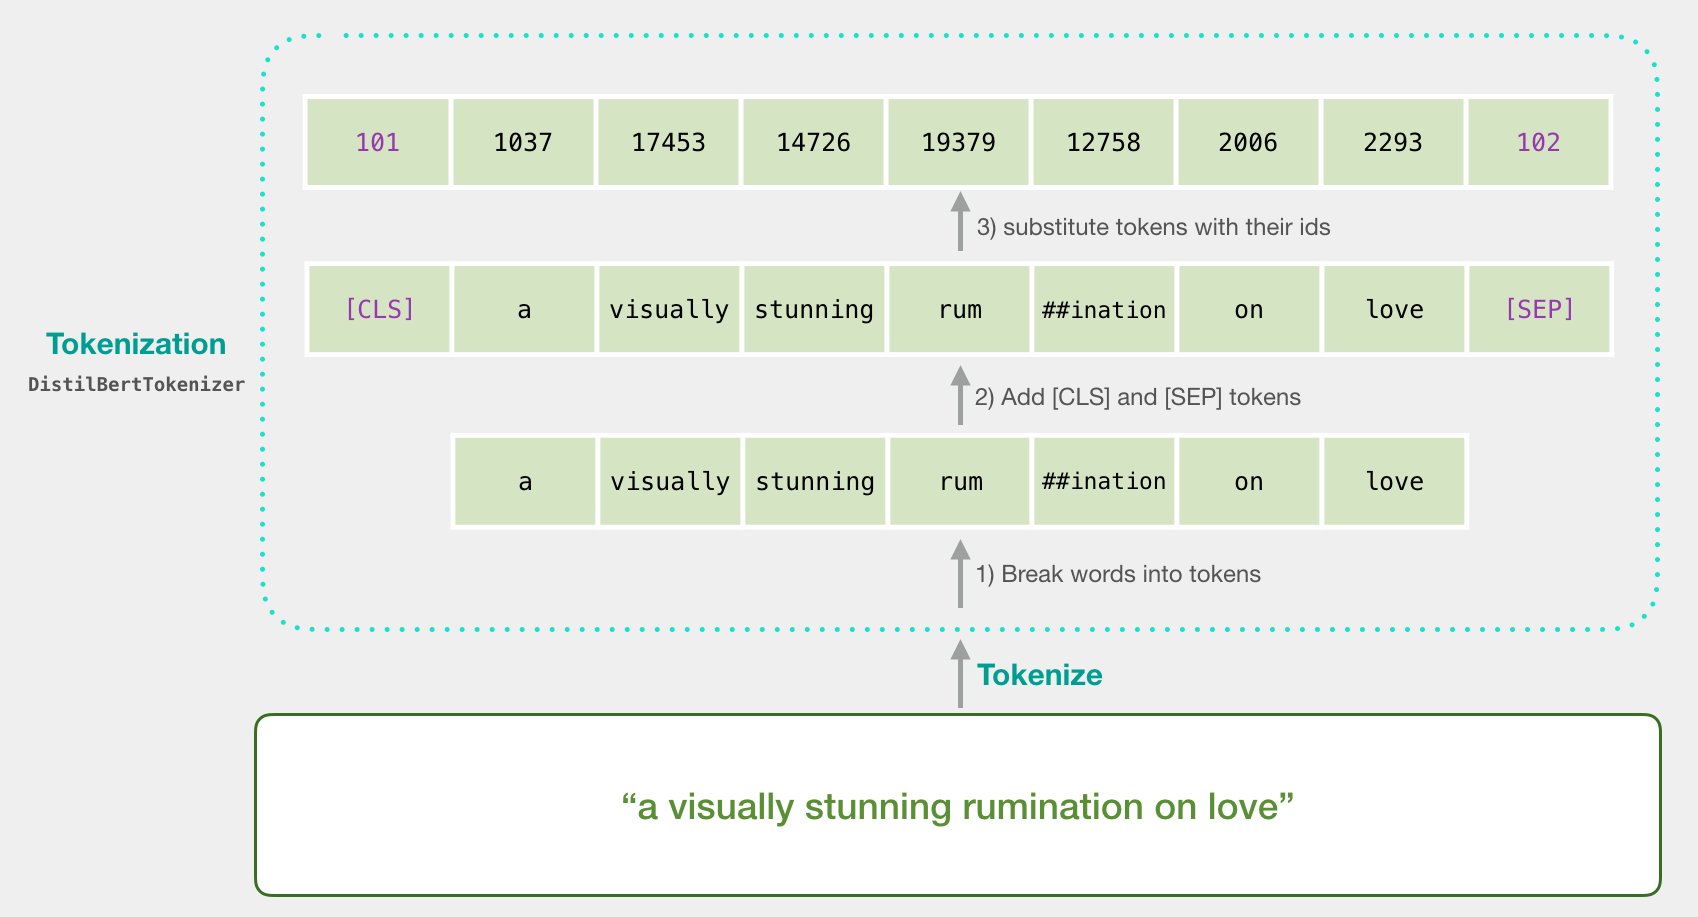
\includegraphics[width=\linewidth]{chapters/NLP/figures/tokenization.png}
    \caption{Tokenization}
    \label{fig:tokenization}
\end{figure}
These steps can be slow and in principle we need to do them only once and cache the results.

\subsubsection{Data Splitting}
\begin{figure}[h]
    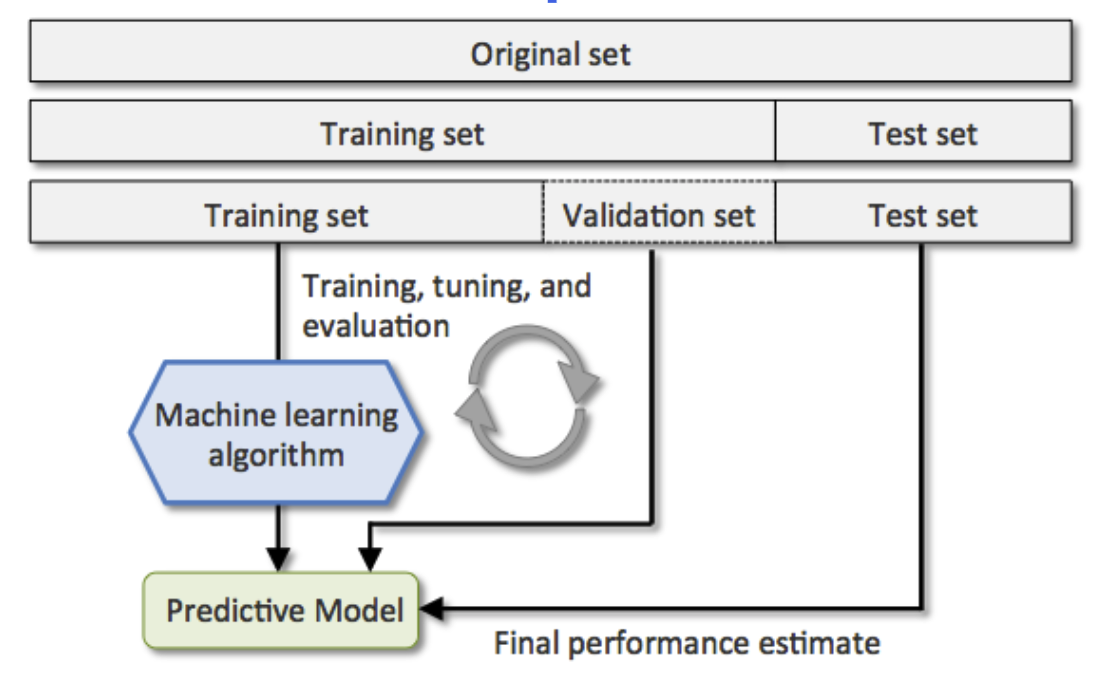
\includegraphics[width=\linewidth]{chapters/NLP/figures/data_splitting.png}
    \caption{Data Splitting}
    \label{fig:data_splitting}
\end{figure}
In order to evaluate the generalization performance of a model it must be tested on data it hasn't seen during training.
The dataset is therefore split into training and validation sets, typically at random (Fig. \ref{fig:data_splitting}).
It should be ensured the randomness is deterministic to reproduce results exactly, which can be achieved by setting a "seed" for the random number generator.
The validation set is used during training to monitor progress and tune hyperparameters.
In addition, it is good practice to hold out another portion of the data, the test set, which is never used during training, but only to report final results.
We otherwise run the risk of tuning hyperparameters to the validation data, thereby overestimating real performance.
% Cross validation?
\subsubsection{Feeding Data to the Model}

\subsection{Metrics and Sanity Checking}
\label{metrics_and_sanity_checking}
We automatically generate metrics and plots relevant for text classification projects.
